%&tex

\documentclass[14pt]{ffslides}

\ffpage{40}{1.7777}

\usepackage{helvet}
\usepackage[english]{babel}
\usepackage[utf8]{inputenc}
\usepackage[T1]{fontenc}
\usepackage{wrapfig}
\usepackage{csquotes}
\usepackage{mathtools}
\usepackage{amsfonts}
\usepackage{amsthm}
\usepackage{amssymb}
\usepackage{thmtools,thm-restate}
\usepackage{multicol}
\usepackage{hyperref}
\usepackage{graphicx}
\usepackage{pifont}
\usepackage[singlelinecheck=false]{caption}
\usepackage{algorithm}
\usepackage[noend]{algpseudocode}
\usepackage{subcaption}
\usepackage{booktabs}
\usepackage{textcomp}
\usepackage{xcolor,colortbl}
\usepackage{enumitem}
\usepackage{multirow}
\usepackage{multicol}
\usepackage{pgfplots}
\usepackage{natbib}
\usepackage{bibentry}
\usepackage{tikz}
\usetikzlibrary{shapes,arrows,positioning,fit,circuits.logic.US}
\pgfplotsset{compat=1.17}

\bibliographystyle{plainnat}

\definecolor{Gray}{gray}{0.5}
\definecolor{Cyan}{rgb}{0.9,1,1}
\definecolor{Yellow}{rgb}{0.7,0.98,0.98}
\definecolor{Red}{rgb}{0.75,0,0}
\definecolor{DarkGreen}{HTML}{10850c}

\definecolor{pdblue}{HTML}{205abd}
\definecolor{ppurple}{HTML}{331832}
\definecolor{pbrickred}{HTML}{D1495B}
\definecolor{psunray}{HTML}{EDAE49}
\definecolor{pmunsell}{HTML}{04A777}

\definecolor{pyellow}{HTML}{FFE066}
\definecolor{pblue}{HTML}{5AB0D5}
\definecolor{pgreen}{HTML}{70C1B3}
\definecolor{porange}{HTML}{DF9F74}
\definecolor{pteal}{HTML}{22C6AB}
\definecolor{pviolet}{HTML}{8332AC}
\definecolor{psandy}{HTML}{6C441E}
\definecolor{pdgreen}{HTML}{219E31}
\definecolor{llw}{rgb}{0.00784313725490196,0.24313725490196078,1.0}
\definecolor{unif}{rgb}{1.0,0.48627450980392156,0.0}
\definecolor{em}{rgb}{0.10196078431372549,0.788235294117647,0.2196078431372549}
\definecolor{stack}{rgb}{0.9098039215686274,0.0,0.043137254901960784}
\definecolor{bmc}{rgb}{0.5450980392156862,0.16862745098039217,0.8862745098039215}
\definecolor{strudel}{rgb}{0.6235294117647059,0.2823529411764706,0.0}
\definecolor{learnpsdd}{rgb}{0.6392156862745098,0.6392156862745098,0.6392156862745098}
\definecolor{learnspn}{rgb}{0.0,0.8431372549019608,1.0}

\newlist{checks}{itemize}{2}
\setlist[checks]{label=$\square$,align=left,labelindent=*}
\newcommand{\cmark}{\ding{51}}%
\newcommand{\xmark}{\ding{55}}%
\newcommand{\done}{\rlap{$\square$}{\raisebox{2pt}{\large\hspace{1pt}\textcolor{DarkGreen}{\cmark}}}}
\newcommand{\wontfix}{\rlap{$\square$}{\large\hspace{1pt}\textcolor{Red}{\xmark}}}

\DeclareMathOperator*{\argmin}{arg\,min}
\DeclareMathOperator*{\argmax}{arg\,max}
\DeclareMathOperator*{\Val}{\text{Val}}
\DeclareMathOperator*{\Ch}{\text{Ch}}
\DeclareMathOperator*{\Pa}{\text{Pa}}
\DeclareMathOperator*{\Sc}{\text{Sc}}
\newcommand{\ov}{\overline}
\newcommand{\tsup}{\textsuperscript}

\newcommand\defeq{\mathrel{\overset{\makebox[0pt]{\mbox{\normalfont\tiny\sffamily def}}}{=}}}

\newcommand{\algorithmautorefname}{Algorithm}
\algrenewcommand\algorithmicrequire{\textbf{Input}}
\algrenewcommand\algorithmicensure{\textbf{Output}}
\algnewcommand{\LineComment}[1]{\State\,\(\triangleright\) #1}

\newcommand{\set}[1]{\mathbf{#1}}
\newcommand{\pr}{\text{P}}
\newcommand{\eps}{\varepsilon}
\newcommand{\ddspn}[2]{\frac{\partial#1}{\partial#2}}
\newcommand{\iddspn}[2]{\partial#1/\partial#2}
\newcommand{\indep}{\perp}
\renewcommand{\implies}{\Rightarrow}

\newcommand{\bigo}{\mathcal{O}}
\newcommand{\mbf}[1]{\mathbf{#1}}

\newcommand{\code}[1]{\lstinline[mathescape=true]{#1}}
\newcommand{\mcode}[1]{\lstinline[mathescape]!#1!}

\DeclareMathOperator{\Sum}{\normalfont{S}}
\DeclareMathOperator{\Sums}{\mathbf{S}}
\DeclareMathOperator{\Prod}{\normalfont{P}}
\DeclareMathOperator{\Prods}{\mathbf{P}}
\DeclareMathOperator{\Leaf}{\normalfont{L}}
\DeclareMathOperator{\Leaves}{\mathbf{L}}
\DeclareMathOperator{\Node}{\normalfont{N}}
\DeclareMathOperator{\Nodes}{\mathbf{N}}
\DeclareMathOperator{\Child}{\normalfont{C}}
\DeclareMathOperator{\Children}{\mathbf{C}}
\DeclareMathOperator{\Conj}{\otimes}
\DeclareMathOperator{\Disj}{\oplus}
\DeclareMathOperator{\Forget}{\normalfont{Forget}}

\newcommand{\newGraphNode}[4]{\node[#4] (#1) at (#2) {\rotatebox{-90}{#3}}}
\newcommand{\newAndNode}[4]{\node[#4,and gate,fill=blue!50!red!30] (#1) at (#2) {\rotatebox{-90}{#3}}}
\newcommand{\newOrNode}[4]{\node[#4,or gate,fill=blue!50!green!30] (#1) at (#2) {\rotatebox{-90}{#3}}}

\newcommand*\llwi{\resizebox{10pt}{!}{\tikz{\node[shape=circle,fill=llw,minimum size=5pt] (char) {};}}}
\newcommand*\unifi{\resizebox{10pt}{!}{\tikz{\node[shape=rectangle,fill=llw,minimum size=8pt] (char) {};}}}
\newcommand*\emi{\resizebox{10pt}{!}{\tikz{\node[shape=diamond,fill=llw,minimum size=8pt] (char) {};}}}
\newcommand*\stacki{\resizebox{10pt}{!}{\tikz{\node[regular polygon,regular polygon sides=3,fill=llw,minimum size=8pt] (char) {};}}}
\newcommand*\bmci{\resizebox{10pt}{!}{\tikz{\node[regular polygon,regular polygon sides=3,rotate=180,fill=llw,minimum size=3pt] (char) {};}}}

\pagenumbering{gobble}

\tikzset{
  every overlay node/.style={
    anchor=north west,
  },
}
\def\tikzoverlay{%
   \tikz[baseline,overlay]\node[every overlay node]
}%

\definecolor{LightGray}{gray}{0.85}

\renewcommand{\familydefault}{\sfdefault}

\geometry{
  left=0.5cm,
  right=0.5cm,
  top=0.5cm,
  bottom=0.5cm,
}

\input{../led}

\begin{document}

% Title
\blankpage

\begin{center}
  \vspace*{\fill}
  \vskip 0.75cm
  \resizebox{\textwidth}{!}{
    \begin{minipage}{0.375\textwidth}
      \begin{center}
        \textcolor{pdblue}{\textbf{Learning Probabilistic Sentential Decision Diagrams\\
          Under Logic Constraints by Sampling and Averaging}}
      \end{center}
    \end{minipage}
  }
  \vskip 1.5cm
  \resizebox{0.8\textwidth}{!}{
    \begin{minipage}{0.25\textwidth}
      \begin{center}
        \textcolor{pdblue}{\textbf{Renato L. Geh}}

        \texttt{renatolg@ime.usp.br}
      \end{center}
    \end{minipage}\hspace{-1cm}\begin{minipage}{0.25\textwidth}
      \begin{center}
        \textcolor{pdblue}{Denis D. Mauá}

        \texttt{ddm@ime.usp.br}
      \end{center}
    \end{minipage}
  }
  \vskip 1.5cm
  \resizebox{0.9\textwidth}{!}{
  \begin{minipage}{0.5\textwidth}
    \color{ppurple}
    \begin{center}
      Department of Computer Science
    \end{center}
    \begin{center}
      Institute of Mathematics and Statistics, University of São Paulo
    \end{center}
  \end{minipage}
  }
  \vskip 1cm
  \begin{center}
    
\includegraphics[width=3cm]{../poster/figures/usp.eps}
  \end{center}
  \vskip 0.5cm
  \resizebox{\textwidth}{!}{
    \begin{minipage}{0.5\textwidth}
      \begin{center}
        \color{pbrickred}\textbf{UAI 2021}
      \end{center}
    \end{minipage}
  }
  \vspace*{\fill}
\end{center}

% PSDDs 1
\newpage

\resizebox{0.8\textwidth}{!}{\textcolor{pdblue}{Probabilistic Sentential Decision Diagrams}}
\vskip 1cm
\resizebox{0.495\textwidth}{!}{
\begin{minipage}{0.39\textwidth}
  \colorbox{pyellow}{\underline{\textbf{P}robabilistic \textbf{S}entential \textbf{D}ecision \textbf{D}iagrams
  (\textbf{PSDD}s):}}
  \begin{itemize} \itemsep0pt %[nosep]
    \item \textcolor{Red}{Structured Decomposable} probabilistic circuits
    \item Encode \textcolor{Red}{certain} knowledge as logic constraints
    \item Encode \textcolor{Red}{uncertain} knowledge as probabilities
    \item \textcolor{Red}{Interpretable} syntax
    \item Many \textcolor{Red}{inferences} are \colorbox{pteal!50}{exact} and \colorbox{pteal!50}{tractable}:
      \setlength{\multicolsep}{1.0pt}
      \begin{multicols}{2}
        \noindent
        \begin{checks}[nosep,label=$\square$]
          \item[\done] Evidence
          \item[\done] Marginals
          \item[\done] MLE Parameter Learning
          \item[\done] Most Probable Explanation
          \item[\done] Expectations
          \item[\done] KL-divergence
        \end{checks}
      \end{multicols}
	\end{itemize}
  \begin{itemize}
	\item PSDD circuit represents recursive decomposition of formula:
      \begin{equation*}
        \bigvee_{i=1}^k (\textcolor{pviolet}{p_i}\wedge\textcolor{psandy}{s_i})\text{, where each
          \emph{prime} \textcolor{pviolet}{$p_i$} and \emph{sub} \textcolor{psandy}{$s_i$} are logical formulae}
      \end{equation*}
	\end{itemize}
\vskip 0.5cm
\hspace{1cm}\textcolor{darkgray}{\cite{darwiche11,kisa14}}

\end{minipage}}\resizebox{0.4\textwidth}{!}{\begin{minipage}{0.35\textwidth}
  \begin{center}
   \resizebox{\textwidth}{!}{
   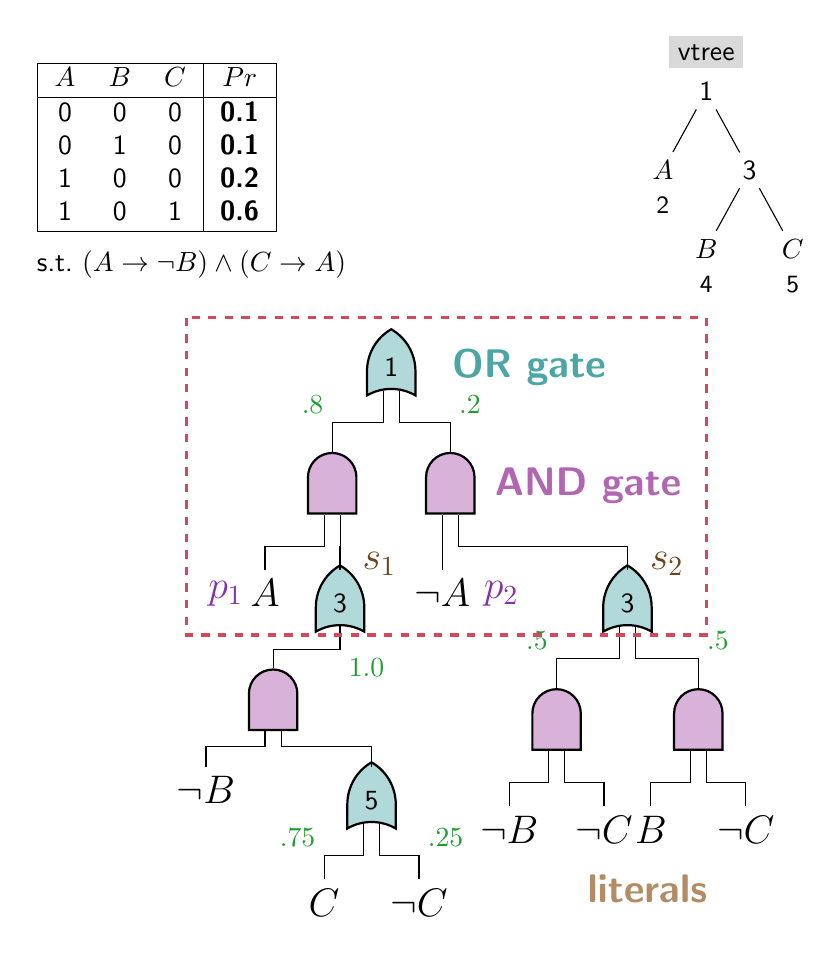
\begin{tikzpicture}[circuit logic US, every circuit symbol/.style={thick}]
     \node (tab) at (-2,2.5) {
     \parbox[c]{5cm}{
       \begin{tabular}{|ccc|c|} \hline
         $A$ & $B$ & $C$ & $Pr$\\
         \hline
         0 & 0 & 0 & \textbf{0.1}\\
         0 & 1 & 0 & \textbf{0.1}\\
         1 & 0 & 0 & \textbf{0.2}\\
         1 & 0 & 1 & \textbf{0.6}\\ \hline
       \end{tabular}\vskip 0.2cm
       s.t.\ $(A\to\neg B)\wedge(C\to A)$}
     };

    \tikzstyle{every node}=[inner sep=3pt]
    \node (v_root) at (4,3.5) {1};
    \node at ($(v_root) + (0,0.5)$) {\colorbox{LightGray}{vtree}};
    \node[label={below:\small 2}] (v_lr) at ($(v_root)+(-0.55, -1.0)$) {$A$};
    \node (v_rr) at ($(v_root)+(0.55,-1.0)$) {3};
    \node[label={below:\small 4}] (v_lrr) at ($(v_root)+(0,-2.0)$) {$B$};
    \node[label={below:\small 5}] (v_rrr) at ($(v_root)+(1.1, -2.0)$) {$C$};
    \draw (v_root) -- (v_lr);
    \draw (v_root) -- (v_rr);
    \draw (v_rr) -- (v_lrr);
    \draw (v_rr) -- (v_rrr);

    \begin{scope}[every node/.style={point up}]
      \newOrNode{r}{0,0}{1}{inputs=nn};
      \newAndNode{p1}{-0.75,-1.5}{}{inputs=nn};
      \newAndNode{p2}{0.75,-1.5}{}{inputs=nn};
      \newOrNode{s1}{-0.65,-3.0}{3}{inputs=nn};
      \newOrNode{s2}{3.0,-3.0}{3}{inputs=nn};
      \newAndNode{s1p1}{-1.5,-4.25}{}{inputs=nn};
      \newAndNode{s2p1}{2.1,-4.5}{}{inputs=nn};
      \newAndNode{s2p2}{3.9,-4.5}{}{inputs=nn};
      \newOrNode{s3}{-0.25,-5.5}{5}{inputs=nn};
    \end{scope}

    \begin{scope}[every node/.style={font=\Large}]
      \node (p1l) at ($(p1.input 1) + (-0.75,-1.0)$) {$A$};
      \node (p2l) at ($(p2.input 1) + (0.0,-1.0)$) {$\neg A$};
      \node (s1p1l) at ($(s1p1.input 1) + (-0.75,-0.75)$) {$\neg B$};
      \node (s2p1l1) at ($(s2p1.input 1) + (-0.5,-1.0)$) {$\neg B$};
      \node (s2p1l2) at ($(s2p1.input 2) + (0.5,-1.0)$) {$\neg C$};
      \node (s2p2l1) at ($(s2p2.input 1) + (-0.5,-1.0)$) {$B$};
      \node (s2p2l2) at ($(s2p2.input 2) + (0.5,-1.0)$) {$\neg C$};
      \node (s3l1) at ($(s3.input 1) + (-0.5,-1.0)$) {$C$};
      \node (s3l2) at ($(s3.input 2) + (0.5,-1.0)$) {$\neg C$};
      \node at ($(r) + (1.75, 0)$) {\color{blue!50!green!70}\textbf{OR gate}};
      \node at ($(p2) + (1.75, 0)$) {\color{blue!50!red!60}\textbf{AND gate}};
      \node at ($(s2p2l2) + (-1.25, -0.75)$) {\color{orange!50!black!60}\textbf{literals}};
    \end{scope}
    \draw (r.input 1) -- ++(0,-0.4) -| node[above left]{\color{pdgreen}$.8$} (p1);
    \draw (r.input 2) -- ++(0,-0.4) -| node[above right]{\color{pdgreen}$.2$} (p2);
    \draw (p1.input 1) -- ++(0,-0.4) -| (p1l);
    \draw (p2.input 1) -- ++(0,-0.4) -| (p2l);
    \draw (s1p1.input 1) -- ++(0,-0.2) -| (s1p1l);
    \draw (s2p1.input 1) -- ++(0,-0.4) -| (s2p1l1);
    \draw (s2p1.input 2) -- ++(0,-0.4) -| (s2p1l2);
    \draw (s2p2.input 1) -- ++(0,-0.4) -| (s2p2l1);
    \draw (s2p2.input 2) -- ++(0,-0.4) -| (s2p2l2);
    \draw (s3.input 1) -- ++(0,-0.4) -| node[above left]{\color{pdgreen}$.75$} (s3l1);
    \draw (s3.input 2) -- ++(0,-0.4) -| node[above right]{\color{pdgreen}$.25$} (s3l2);
    \draw (p1.input 2) -- ++(0,-0.4) -| (s1);
    \draw (p2.input 2) -- ++(0,-0.4) -| (s2);
    \draw (s1.west) -- ++(0,-0.3) node[below right]{\color{pdgreen}$1.0$} -| (s1p1);
    \draw (s2.input 1) -- ++(0,-0.4) -| node[above left]{\color{pdgreen}$.5$} (s2p1);
    \draw (s2.input 2) -- ++(0,-0.4) -| node[above right]{\color{pdgreen}$.5$} (s2p2);
    \draw (s1p1.input 2) -- ++ (0,-0.2) -| (s3);

    \draw[very thick,dashed,pbrickred] ($(p1l) + (-1.0,3.5)$) rectangle ($(s2) + (1.0,-0.4)$);
    \node at ($(p1l) + (-0.5,0)$) {\color{pviolet}\Large$p_1$};
    \node at ($(s1) + (0.5,0.5)$) {\color{psandy}\Large$s_1$};
    \node at ($(p2l) + (0.75,0.0)$) {\color{pviolet}\Large$p_2$};
    \node at ($(s2) + (0.5,0.5)$) {\color{psandy}\Large$s_2$};
  \end{tikzpicture}
  }
\end{center}
\end{minipage}}

% PSDDs 2

\newpage
\resizebox{0.8\textwidth}{!}{\textcolor{pdblue}{Probabilistic Sentential Decision Diagrams}}
\vskip 0.25cm
\resizebox{0.49\textwidth}{!}{
\begin{minipage}{0.39\textwidth}
  \colorbox{pyellow}{\underline{\textbf{Existing PSDD learners:}}}
  \vskip 0.25cm
  \textsc{LearnPSDD} (\textcolor{darkgray}{\cite{liang17}}):
  \begin{checks}
    \item[\wontfix] Requires initial PSDD encoding the support...
    \item[\wontfix] Scales poorly to complex formulae and/or high dimension...
    \item[\wontfix] Costly whole circuit evaluation at every iteration...
    \item[\done] Very good performance!
  \end{checks}
  \textsc{Strudel} (\textcolor{darkgray}{\cite{mei20}}):
  \begin{checks}
    \item[\done] Constructs an initial PSDD structure (from a CLT)!
    \item[\wontfix] But does not encode constraints...
    \item[\done] Scales to high dimension!
    \item[\wontfix] As long as the circuit doesn't get too big...
  \end{checks}
  \textsc{SamplePSDD} (this work):
  \begin{checks}
    \item[\done] Scales to high dimension and complex formulae!
    \item[\done] Constructs a structure consistent with constraints!
    \item[\wontfix] But does so by relaxing the formula...
    \item[\wontfix] Performance varies on set bounds and vtree structure...
  \end{checks}
  %\hspace{0.5cm}\textcolor{darkgray}{\cite{mattei19,geh20}}
\end{minipage}}\resizebox{0.4\textwidth}{!}{\begin{minipage}{0.35\textwidth}
  \begin{center}
    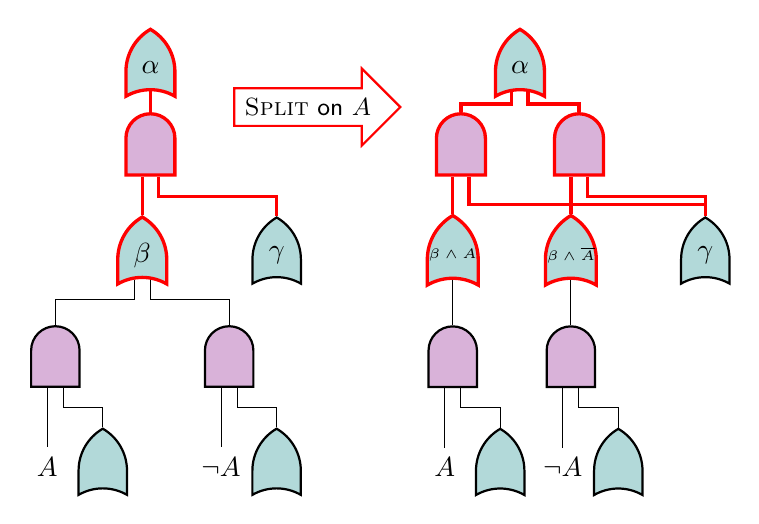
\begin{tikzpicture}[circuit logic US]
      \begin{scope}[every node/.style={point up}]
        \begin{scope}[every circuit symbol/.style={draw=red,very thick}]
          \newOrNode{r}{0,0}{$\alpha$}{inputs=nn};
          \newAndNode{p1}{0,-1}{}{inputs=nn};
          \newOrNode{s1}{$(p1.input 1) + (0,-1)$}{$\beta$}{inputs=nn};
        \end{scope}
        \begin{scope}[every circuit symbol/.style={thick}]
          \newOrNode{s2}{$(p1.input 2) + (1.5,-1)$}{$\gamma$}{inputs=nn};
          \newAndNode{p2}{$(s1.input 1) + (-1.0,-1)$}{}{inputs=nn};
          \newAndNode{p3}{$(s1.input 2) + (1.0,-1)$}{}{inputs=nn};
          \newOrNode{s3}{$(p2.input 2) + (0.5,-1)$}{}{inputs=nn};
          \newOrNode{s4}{$(p3.input 2) + (0.5,-1)$}{}{inputs=nn};
        \end{scope}
    \end{scope}
    \node (a) at ($(p2.input 1) + (0.0,-1)$) {$A$};
    \node (na) at ($(p3.input 1) + (0.0,-1)$) {$\neg A$};
    \draw[draw=red,very thick] (r.west) -- (p1.east);
    \draw[draw=red,very thick] (p1.input 1) -- (s1.east);
    \draw[draw=red,very thick] (p1.input 2) -- ++(0,-0.25) -| (s2.east);
    \draw (s1.input 1) -- ++(0,-0.25) -| (p2.east);
    \draw (s1.input 2) -- ++(0,-0.25) -| (p3.east);
    \draw (p2.input 1) -- (a);
    \draw (p2.input 2) -- ++(0,-0.25) -| (s3.east);
    \draw (p3.input 1) -- (na);
    \draw (p3.input 2) -- ++(0,-0.25) -| (s4.east);

    \node[style={single arrow,draw=red,thick}] (arrow) at (2,-0.5)
      {\small\textrm{\textsc{Split}} on $A$};

    \begin{scope}[every node/.style={point up}]
      \begin{scope}[every circuit symbol/.style={draw=red,very thick}]
        \newOrNode{r}{$(arrow.east) + (1.5,0.5)$}{$\alpha$}{inputs=nn};
        \newAndNode{p1}{$(r) + (0.75,-1)$}{}{inputs=nn};
        \newAndNode{p12}{$(r) + (-0.75,-1)$}{}{inputs=nn};
        \newOrNode{s1}{$(p1.input 1) + (0,-1)$}{\tiny$\beta\wedge\overline{A}$}{inputs=nn};
        \newOrNode{s12}{$(p12.input 1) + (0,-1)$}{\tiny$\beta\wedge A$}{inputs=nn};
      \end{scope}
      \begin{scope}[every circuit symbol/.style={thick}]
        \newOrNode{s2}{$(p1.input 2) + (1.5,-1)$}{$\gamma$}{inputs=nn};
        \newAndNode{p2}{$(s12.west) + (0,-1)$}{}{inputs=nn};
        \newAndNode{p3}{$(s1.west) + (0,-1)$}{}{inputs=nn};
        \newOrNode{s3}{$(p2.input 2) + (0.5,-1)$}{}{inputs=nn};
        \newOrNode{s4}{$(p3.input 2) + (0.5,-1)$}{}{inputs=nn};
      \end{scope}
    \end{scope}
    \node (a) at ($(p2.input 1) + (0.0,-1)$) {$A$};
    \node (na) at ($(p3.input 1) + (0.0,-1)$) {$\neg A$};
    \draw[draw=red,very thick] (r.input 1) -- ++(0,-0.15) -| (p12.east);
    \draw[draw=red,very thick] (r.input 2) -- ++(0,-0.15) -| (p1.east);
    \draw[draw=red,very thick] (p1.input 1) -- (s1.east);
    \draw[draw=red,very thick] (p1.input 2) -- ++(0,-0.25) -| (s2.east);
    \draw[draw=red,very thick] (p12.input 2) -- ++(0,-0.35) -| (s2.east);
    \draw[draw=red,very thick] (p12.input 1) -- (s12.east);
    \draw (s12.west) -- ++(0,-0.25) -| (p2.east);
    \draw (s1.west) -- ++(0,-0.25) -| (p3.east);
    \draw (p2.input 1) -- (a);
    \draw (p2.input 2) -- ++(0,-0.25) -| (s3.east);
    \draw (p3.input 1) -- (na);
    \draw (p3.input 2) -- ++(0,-0.25) -| (s4.east);
  \end{tikzpicture}
  \vskip 0.5cm
  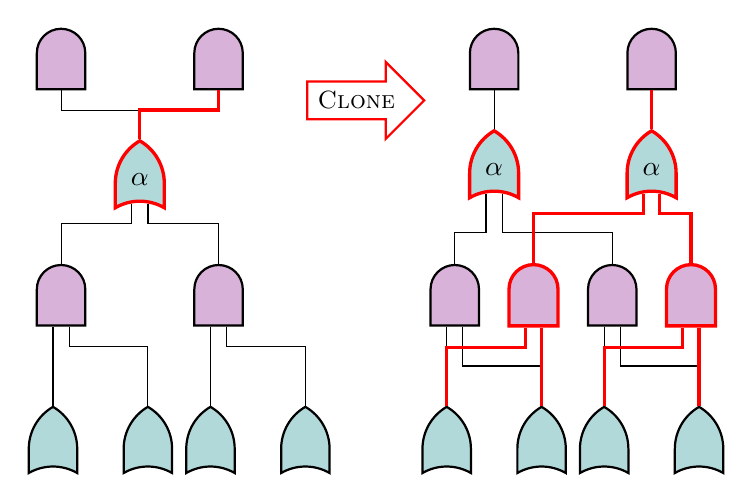
\begin{tikzpicture}[circuit logic US]
    \begin{scope}[every node/.style={point up}]
      \begin{scope}[every circuit symbol/.style={draw=red,very thick}]
        \newOrNode{s1}{0,-1.5}{$\alpha$}{inputs=nn};
      \end{scope}
      \begin{scope}[every circuit symbol/.style={thick}]
        \newAndNode{r1}{-1,0}{}{inputs=nn};
        \newAndNode{r2}{1,0}{}{inputs=nn};
        \newAndNode{p1}{$(r1)+(0,-3)$}{}{inputs=nn};
        \newAndNode{p2}{$(r2)+(0,-3)$}{}{inputs=nn};
        \newOrNode{l11}{$(p1.input 1)+(0,-1.5)$}{}{inputs=nn};
        \newOrNode{l12}{$(p1.input 2)+(1,-1.5)$}{}{inputs=nn};
        \newOrNode{l21}{$(p2.input 1)+(0,-1.5)$}{}{inputs=nn};
        \newOrNode{l22}{$(p2.input 2)+(1,-1.5)$}{}{inputs=nn};
      \end{scope}
    \end{scope}
    \draw (r1.west) -- ++(0,-0.25) -| (s1.east);
    \draw[draw=red,very thick] (r2.west) -- ++(0,-0.25) -| (s1.east);
    \draw (s1.input 1) -- ++(0,-0.25) -| (p1.east);
    \draw (s1.input 2) -- ++(0,-0.25) -| (p2.east);
    \draw (p1.input 1) -- ++(0,-0.25) -| (l11.east);
    \draw (p1.input 2) -- ++(0,-0.25) -| (l12.east);
    \draw (p2.input 1) -- ++(0,-0.25) -| (l21.east);
    \draw (p2.input 2) -- ++(0,-0.25) -| (l22.east);

    \node[style={single arrow,draw=red,thick}] (arrow) at (2.75,-0.5)
      {\small\textrm{\textsc{Clone}}};

    \begin{scope}[every node/.style={point up}]
      \begin{scope}[every circuit symbol/.style={thick}]
        \newAndNode{r1}{4.5,0}{}{inputs=nn};
        \newAndNode{r2}{6.5,0}{}{inputs=nn};
        \newAndNode{p1}{$(r1)+(-0.5,-3)$}{}{inputs=nn};
        \newAndNode{p2}{$(r2)+(-0.5,-3)$}{}{inputs=nn};
        \newOrNode{l11}{$(p1.input 1)+(0,-1.5)$}{}{inputs=nn};
        \newOrNode{l12}{$(p1.input 2)+(1,-1.5)$}{}{inputs=nn};
        \newOrNode{l21}{$(p2.input 1)+(0,-1.5)$}{}{inputs=nn};
        \newOrNode{l22}{$(p2.input 2)+(1,-1.5)$}{}{inputs=nn};
      \end{scope}
      \begin{scope}[every circuit symbol/.style={draw=red,very thick}]
        \newOrNode{s1}{$(r1.west) + (0,-1)$}{$\alpha$}{inputs=nn};
        \newOrNode{s2}{$(r2.west) + (0,-1)$}{$\alpha$}{inputs=nn};
        \newAndNode{p3}{$(p1)+(1,0)$}{}{inputs=nn};
        \newAndNode{p4}{$(p2)+(1,0)$}{}{inputs=nn};
      \end{scope}
    \end{scope}
    \draw (r1.west) -- ++(0,-0.25) -| (s1.east);
    \draw[draw=red,very thick] (r2.west) -- ++(0,-0.25) -| (s2.east);
    \draw (s1.input 1) -- ++(0,-0.5) -| (p1.east);
    \draw (s1.input 2) -- ++(0,-0.5) -| (p2.east);
    \draw[draw=red,very thick] (s2.input 1) -- ++(0,-0.25) -| (p3.east);
    \draw[draw=red,very thick] (s2.input 2) -- ++(0,-0.25) -| (p4.east);
    \draw (p1.input 1) -- ++(0,-0.25) -| (l11.east);
    \draw (p1.input 2) -- ++(0,-0.5) -| (l12.east);
    \draw (p2.input 1) -- ++(0,-0.25) -| (l21.east);
    \draw (p2.input 2) -- ++(0,-0.5) -| (l22.east);
    \draw[draw=red,very thick] (p3.input 1) -- ++(0,-0.25) -| (l11.east);
    \draw[draw=red,very thick] (p3.input 2) -- ++(0,-0.5) -| (l12.east);
    \draw[draw=red,very thick] (p4.input 1) -- ++(0,-0.25) -| (l21.east);
    \draw[draw=red,very thick] (p4.input 2) -- ++(0,-0.5) -| (l22.east);
  \end{tikzpicture}
\end{center}
\end{minipage}}

% SamplePSDD 1
\newpage
\resizebox{0.275\textwidth}{!}{\textcolor{pdblue}{\textsc{SamplePSDD}}}
\vskip 1cm
\begin{center}
\resizebox{0.6\textwidth}{!}{
   \textcolor{Red}{Common assumption}: primes \textcolor{pviolet}{$p_i$} are \colorbox{pblue}{conjunctions of literals}.
}
\vskip 1cm
\resizebox{0.6\textwidth}{!}{
  $\phi(A,B,C,D)=(A\wedge\neg B\wedge\neg D)\vee(B\wedge\neg C \wedge D)$
}
\vskip 1cm
\resizebox{0.6\textwidth}{!}{
  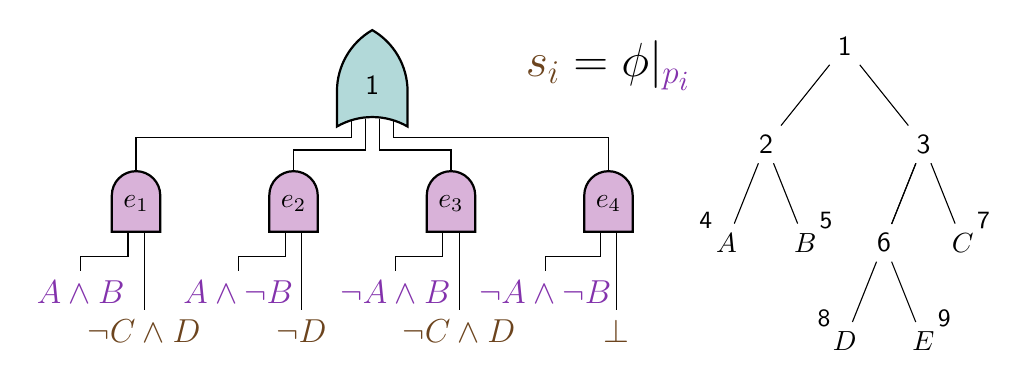
\begin{tikzpicture}[circuit logic US, every circuit symbol/.style={thick}]
    \begin{scope}[every node/.style={point up}]
      \newOrNode{r}{0,0}{1}{inputs=nnnn};
      \newAndNode{a1}{$(r) + (-3.0,-1.5)$}{$e_1$}{inputs=nn};
      \newAndNode{a2}{$(r) + (-1.0,-1.5)$}{$e_2$}{inputs=nn};
      \newAndNode{a3}{$(r) + (1.0,-1.5)$}{$e_3$}{inputs=nn};
      \newAndNode{a4}{$(r) + (3.0,-1.5)$}{$e_4$}{inputs=nn};
    \end{scope}
    \begin{scope}[every node/.style={font=\large}]
      \node (p1) at ($(a1.input 1) + (-0.6,-0.75)$) {\color{pviolet}$A\wedge B$};
      \node (p2) at ($(a2.input 1) + (-0.6,-0.75)$) {\color{pviolet}$A\wedge\neg B$};
      \node (p3) at ($(a3.input 1) + (-0.6,-0.75)$) {\color{pviolet}$\neg A\wedge B$};
      \node (p4) at ($(a4.input 1) + (-0.7,-0.75)$) {\color{pviolet}$\neg A\wedge\neg B$};
      \node (s1) at ($(a1.input 2) + (0,-1.25)$) {\color{psandy}$\neg C\wedge D$};
      \node (s2) at ($(a2.input 2) + (0,-1.25)$) {\color{psandy}$\neg D$};
      \node (s3) at ($(a3.input 2) + (0,-1.25)$) {\color{psandy}$\neg C\wedge D$};
      \node (s4) at ($(a4.input 2) + (0,-1.25)$) {\color{psandy}$\bot$};
      \node at ($(r) + (3,0.25)$) {\LARGE$\textcolor{psandy}{s_i}=\phi|_{\textcolor{pviolet}{p_i}}$};
    \end{scope}
    \draw (r.input 1) -- ++(0,-0.2) -| (a1);
    \draw (r.input 2) -- ++(0,-0.4) -| (a2);
    \draw (r.input 3) -- ++(0,-0.4) -| (a3);
    \draw (r.input 4) -- ++(0,-0.2) -| (a4);
    \draw (a1.input 1) -- ++(0,-0.3) -| (p1);
    \draw (a2.input 1) -- ++(0,-0.3) -| (p2);
    \draw (a3.input 1) -- ++(0,-0.3) -| (p3);
    \draw (a4.input 1) -- ++(0,-0.3) -| (p4);
    \draw (a1.input 2) -- ++(0,-0.4) -| (s1);
    \draw (a2.input 2) -- ++(0,-0.4) -| (s2);
    \draw (a3.input 2) -- ++(0,-0.4) -| (s3);
    \draw (a4.input 2) -- ++(0,-0.4) -| (s4);

    \node (root) at (6,0.5) {1};
    \node (nr) at ($(root) + (-1.0,-1.25)$) {2};
    \node (n1) at ($(root) + (1.0,-1.25)$) {3};
    \node[label={[label distance=-7.5pt] above left:\small 4}] (n2) at ($(nr) + (-0.5,-1.25)$) {$A$};
    \node[label={[label distance=-7.5pt] above right:\small 5}] (ne) at ($(nr) + (0.5,-1.25)$) {$B$};
    \node (n3) at ($(n1) + (-0.5,-1.25)$) {6};
    \node[label={[label distance=-7.5pt] above right:\small 7}] (n4) at ($(n1) + (0.5,-1.25)$) {$C$};
    \node[label={[label distance=-7.5pt] above left:\small 8}] (n5) at ($(n3) + (-0.5,-1.25)$) {$D$};
    \node[label={[label distance=-7.5pt] above right:\small 9}] (n6) at ($(n3) + (0.5,-1.25)$) {$E$};
    \draw (root) -- (n1);
    \draw (n1) -- (n3);
    \draw (root) -- (nr);
    \draw (nr) -- (n2);
    \draw (nr) -- (ne);
    \draw (n1) -- (n3);
    \draw (n1) -- (n4);
    \draw (n3) -- (n6);
    \draw (n3) -- (n5);
  \end{tikzpicture}
  }
  \vskip 1cm
  \begin{minipage}{0.55\textwidth}
  \resizebox{\textwidth}{!}{
    \begin{minipage}{0.6\textwidth}
      \colorbox{pyellow}{\textbf{Problem:}} size of circuit is \textcolor{Red}{exponential} in the size of \textcolor{pviolet}{$p_i$}
    \end{minipage}
  }
  \end{minipage}
\end{center}

% SamplePSDD 2
\newpage
\resizebox{0.275\textwidth}{!}{\textcolor{pdblue}{\textsc{SamplePSDD}}}
\vskip 1cm
\begin{center}
  \begin{minipage}{0.55\textwidth}
    \resizebox{\textwidth}{!}{
      \begin{minipage}{0.6\textwidth}
        \colorbox{pteal!50}{\textbf{{Solution:}}} randomly sample a bounded number ($k$) of   \textcolor{pviolet}{$p_i$}
      \end{minipage}
    }
  \end{minipage}
  \vskip 1cm
  \begin{center}
    \resizebox{0.7\textwidth}{!}{
      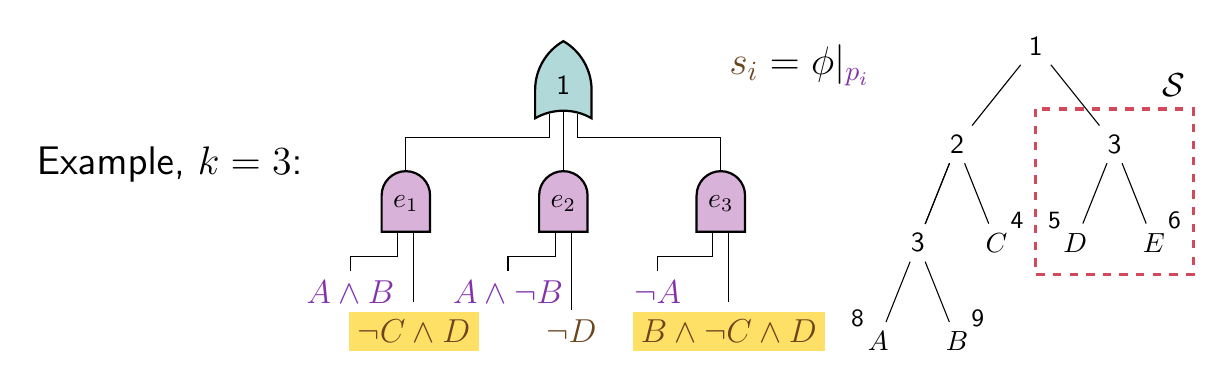
\begin{tikzpicture}[circuit logic US, every circuit symbol/.style={thick}]
        \node at (-5, -1) {\Large Example, $k=3$:};

        \begin{scope}[every node/.style={point up}]
          \newOrNode{r}{0,0}{1}{inputs=nnn};
          \newAndNode{a1}{$(r) + (-2.0,-1.5)$}{$e_1$}{inputs=nn};
          \newAndNode{a2}{$(r) + (0.0,-1.5)$}{$e_2$}{inputs=nn};
          \newAndNode{a3}{$(r) + (2.0,-1.5)$}{$e_3$}{inputs=nn};
        \end{scope}
        \begin{scope}[every node/.style={font=\large}]
          \node (p1) at ($(a1.input 1) + (-0.6,-0.75)$) {\color{pviolet}$A\wedge B$};
          \node (p2) at ($(a2.input 1) + (-0.6,-0.75)$) {\color{pviolet}$A\wedge\neg B$};
          \node (p3) at ($(a3.input 1) + (-0.7,-0.75)$) {\color{pviolet}$\neg A$};
          \node (s1) at ($(a1.input 2) + (0,-1.25)$) {\colorbox{pyellow}{\color{psandy}$\neg C\wedge D$}};
          \node (s2) at ($(a2.input 2) + (0,-1.25)$) {\color{psandy}$\neg D$};
          \node (s3) at ($(a3.input 2) + (0,-1.25)$) {\colorbox{pyellow}{\color{psandy}$B\wedge\neg C\wedge D$}};
          \node at ($(r) + (3,0.25)$) {\Large$\textcolor{psandy}{s_i}=\phi|_{\textcolor{pviolet}{p_i}}$};
        \end{scope}
        \draw (r.input 1) -- ++(0,-0.3) -| (a1);
        \draw (r.input 2) -- ++(0,-0.3) -| (a2);
        \draw (r.input 3) -- ++(0,-0.3) -| (a3);
        \draw (a1.input 1) -- ++(0,-0.3) -| (p1);
        \draw (a2.input 1) -- ++(0,-0.3) -| (p2);
        \draw (a3.input 1) -- ++(0,-0.3) -| (p3);
        \draw (a1.input 2) -- ++(0,-0.4) -| (s1);
        \draw (a2.input 2) -- ++(0,-0.4) -| (s2);
        \draw (a3.input 2) -- ++(0,-0.4) -| (s3);

        \node (root) at (6,0.5) {1};
        \node (n1) at ($(root) + (-1.0,-1.25)$) {2};
        \node (nr) at ($(root) + (1.0,-1.25)$) {3};
        \node[label={[label distance=-7.5pt] above left:\small 5}] (n2) at ($(nr) + (-0.5,-1.25)$) {$D$};
        \node[label={[label distance=-7.5pt] above right:\small 6}] (ne) at ($(nr) + (0.5,-1.25)$) {$E$};
        \node (n3) at ($(n1) + (-0.5,-1.25)$) {3};
        \node[label={[label distance=-7.5pt] above right:\small 4}] (n4) at ($(n1) + (0.5,-1.25)$) {$C$};
        \node[label={[label distance=-7.5pt] above left:\small 8}] (n5) at ($(n3) + (-0.5,-1.25)$) {$A$};
        \node[label={[label distance=-7.5pt] above right:\small 9}] (n6) at ($(n3) + (0.5,-1.25)$) {$B$};
        \draw (root) -- (n1);
        \draw (n1) -- (n3);
        \draw (root) -- (nr);
        \draw (nr) -- (n2);
        \draw (nr) -- (ne);
        \draw (n1) -- (n3);
        \draw (n1) -- (n4);
        \draw (n3) -- (n6);
        \draw (n3) -- (n5);
        \draw[very thick,dashed,pbrickred] ($(n2) + (-0.5,1.7)$) rectangle ($(ne) + (0.5,-0.4)$);
        \node at ($(nr) + (0.75,0.75)$) {\large$\mathcal{S}$};
      \end{tikzpicture}
    }
  \end{center}
  \vskip 1cm
  \begin{minipage}{0.55\textwidth}
    \resizebox{\textwidth}{!}{
      \begin{minipage}{0.6\textwidth}
        \colorbox{pyellow}{\textbf{But:}} this \textcolor{Red}{violates structure} decomposability
      \end{minipage}
    }
  \end{minipage}
  \vskip 1cm
  \begin{minipage}{0.5\textwidth}
    \resizebox{\textwidth}{!}{
      \begin{minipage}{0.6\textwidth}
        \textcolor{psandy}{$\neg C\wedge D$} contains $C$, and $C\not\in\mathcal{S}$

        \textcolor{psandy}{$\neg B\wedge\neg C\wedge D$} contains $B$ and $C$, and $B,C\not\in\mathcal{S}$
      \end{minipage}
    }
  \end{minipage}
\end{center}

% SamplePSDD 4
\newpage
\resizebox{0.275\textwidth}{!}{\textcolor{pdblue}{\textsc{SamplePSDD}}}
\vskip 1cm
\begin{center}
\begin{minipage}{0.4\textwidth}
  \resizebox{\textwidth}{!}{
    \begin{minipage}{0.6\textwidth}
      \colorbox{pteal!50}{\textbf{New solution:}}  relax logical constraints $\phi$
    \end{minipage}
  }
\end{minipage}
\vskip 1.0cm
\begin{center}
\resizebox{0.65\textwidth}{!}{
  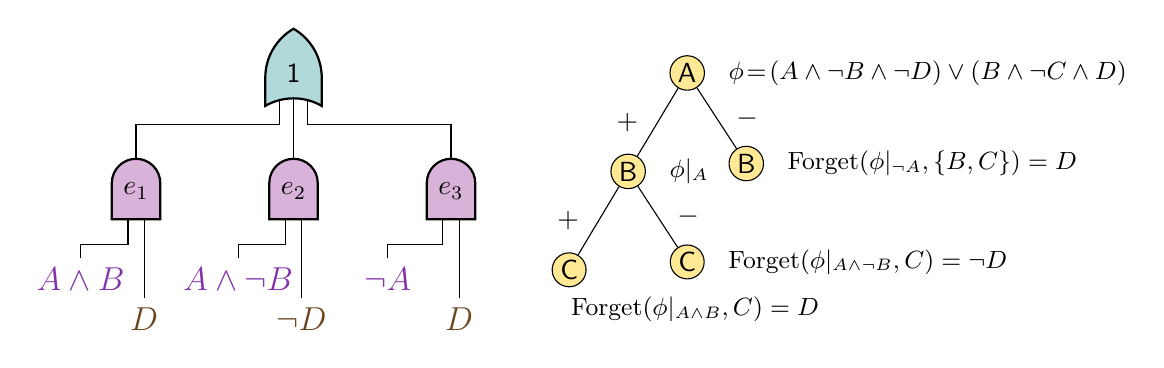
\begin{tikzpicture}[circuit logic US, every circuit symbol/.style={thick}]
    \begin{scope}[every node/.style={point up}]
      \newOrNode{r}{0,0}{1}{inputs=nnn};
      \newAndNode{a1}{$(r) + (-2.0,-1.5)$}{$e_1$}{inputs=nn};
      \newAndNode{a2}{$(r) + (0.0,-1.5)$}{$e_2$}{inputs=nn};
      \newAndNode{a3}{$(r) + (2.0,-1.5)$}{$e_3$}{inputs=nn};
    \end{scope}
    \begin{scope}[every node/.style={font=\large}]
      \node (p1) at ($(a1.input 1) + (-0.6,-0.75)$) {\color{pviolet}$A\wedge B$};
      \node (p2) at ($(a2.input 1) + (-0.6,-0.75)$) {\color{pviolet}$A\wedge\neg B$};
      \node (p3) at ($(a3.input 1) + (-0.7,-0.75)$) {\color{pviolet}$\neg A$};
      \node (s1) at ($(a1.input 2) + (0,-1.25)$) {\color{psandy}$D$};
      \node (s2) at ($(a2.input 2) + (0,-1.25)$) {\color{psandy}$\neg D$};
      \node (s3) at ($(a3.input 2) + (0,-1.25)$) {\color{psandy}$D$};
    \end{scope}
    \draw (r.input 1) -- ++(0,-0.3) -| (a1);
    \draw (r.input 2) -- ++(0,-0.3) -| (a2);
    \draw (r.input 3) -- ++(0,-0.3) -| (a3);
    \draw (a1.input 1) -- ++(0,-0.3) -| (p1);
    \draw (a2.input 1) -- ++(0,-0.3) -| (p2);
    \draw (a3.input 1) -- ++(0,-0.3) -| (p3);
    \draw (a1.input 2) -- ++(0,-0.4) -| (s1);
    \draw (a2.input 2) -- ++(0,-0.4) -| (s2);
    \draw (a3.input 2) -- ++(0,-0.4) -| (s3);
    \begin{scope}
      \tikzstyle{dec} = [draw,circle,inner sep=1pt,fill=pyellow!70];
      \node[dec,label={[label distance=5pt] right:\small$\phi\!=\!(A\wedge \neg B \wedge \neg D) \vee (B \wedge \neg C \wedge D)$}] (root) at (5,0) {A};
      \node[dec] (n1) at ($(root) + (+0.75,-1.15)$) {B};
      \node[dec,label={[label distance=5pt] right:\small$\phi|_{A}$}] (n2) at ($(root) + (-0.75,-1.25)$) {B};
      \node[dec] (n3) at ($(n2) + (+0.75,-1.15)$) {C};
      \node[dec] (n4) at ($(n2) + (-0.75,-1.25)$) {C};
      \draw (root) edge node[label={right:$-$}] {} (n1);
      \draw (root) edge node[label={left:$+$}] {} (n2);
      \draw (n2) edge node[label={right:$-$}] {} (n3);
      \draw (n2) edge node[label={left:$+$}] {} (n4);

     \node[anchor=west]  at ($(n1) + (0.4,0)$) {\small $\Forget(\phi|_{\neg A}, \{B,C\})=D$};
     \node[anchor=west]  at ($(n3) + (+0.4,0)$) {\small $\Forget(\phi|_{A \wedge \neg B}, C)=\neg D$};
     \node[anchor=west]  at ($(n4) + (-0.1,-0.5)$) {\small $\Forget(\phi|_{A \wedge B}, C)=D$};
   \end{scope}
 \end{tikzpicture}
}
\end{center}
\begin{center}
  \resizebox{0.5\textwidth}{!}{
  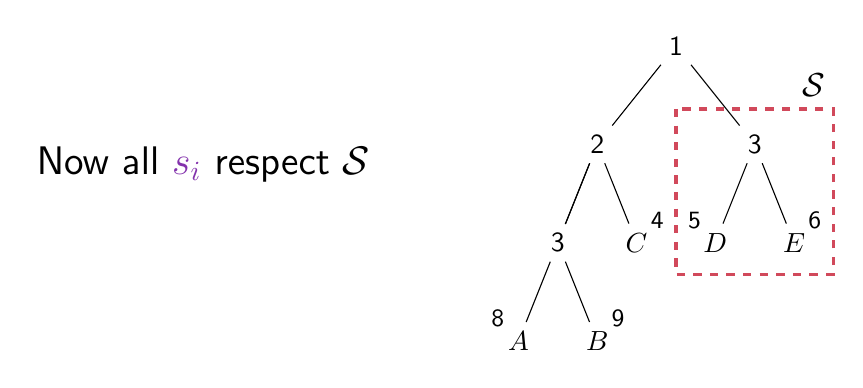
\begin{tikzpicture}
    \node (root) at (6,0.0) {1};
    \node at ($(root) + (-6,-1.5)$) {\Large{}Now all \textcolor{pviolet}{$s_i$} respect $\mathcal{S}$};
    \node (n1) at ($(root) + (-1.0,-1.25)$) {2};
    \node (nr) at ($(root) + (1.0,-1.25)$) {3};
    \node[label={[label distance=-7.5pt] above left:\small 5}] (n2) at ($(nr) + (-0.5,-1.25)$) {$D$};
    \node[label={[label distance=-7.5pt] above right:\small 6}] (ne) at ($(nr) + (0.5,-1.25)$) {$E$};
    \node (n3) at ($(n1) + (-0.5,-1.25)$) {3};
    \node[label={[label distance=-7.5pt] above right:\small 4}] (n4) at ($(n1) + (0.5,-1.25)$) {$C$};
    \node[label={[label distance=-7.5pt] above left:\small 8}] (n5) at ($(n3) + (-0.5,-1.25)$) {$A$};
    \node[label={[label distance=-7.5pt] above right:\small 9}] (n6) at ($(n3) + (0.5,-1.25)$) {$B$};
    \draw (root) -- (n1);
    \draw (n1) -- (n3);
    \draw (root) -- (nr);
    \draw (nr) -- (n2);
    \draw (nr) -- (ne);
    \draw (n1) -- (n3);
    \draw (n1) -- (n4);
    \draw (n3) -- (n6);
    \draw (n3) -- (n5);
    \draw[very thick,dashed,pbrickred] ($(n2) + (-0.5,1.7)$) rectangle ($(ne) + (0.5,-0.4)$);
    \node at ($(nr) + (0.75,0.75)$) {\large$\mathcal{S}$};
  \end{tikzpicture}
  }
\end{center}
\end{center}

% Experiments 1
\newpage
\resizebox{0.25\textwidth}{!}{\textcolor{pdblue}{Experiments}}
\vskip 0.25cm
\resizebox{0.495\textwidth}{!}{
\begin{minipage}{0.39\textwidth}
  \noindent
  \colorbox{pyellow}{\textbf{\underline{Evaluation:}}} we sample 30 PSDDs and use 5 ensemble strategies:
  \vskip 0.25cm
  \begin{enumerate}[nosep]
    \item[\llwi] \textcolor{llw}{\textbf{Likelihood weighting (LLW)}},
    \item[\unifi] \textcolor{llw}{\textbf{Uniform weights}},
    \item[\emi] \textcolor{llw}{\textbf{Expectation Maximization (EM)}},
    \item[\stacki] \textcolor{llw}{\textbf{Stacking}},
    \item[\bmci] \textcolor{llw}{\textbf{Bayesian Model Combination (BMC)}};
  \end{enumerate}
  \vskip 0.25cm
  \hskip 0.25cm comparing against \textcolor{unif}{\textbf{\textsc{Strudel}}},
    \textcolor{unif}{\textbf{\textsc{LearnPSDD}}} and \textcolor{unif}{\textbf{\textsc{LearnSPN}}}.
  \vskip 0.25cm
  \colorbox{pyellow}{\textbf{\underline{Datasets:}}} we evaluate with 5 data + knowledge as logic constraints:
  \vskip 0.25cm
  \begin{center}
    \begin{tabular}{cl|rrrr}
      \cline{2-5}
      &\textbf{Dataset} & \textbf{\#vars} & \textbf{\#train} & \textbf{$\phi$'s size}\\
      \cline{2-5}
      $\Rightarrow$&\textsc{LED} & 14 & 5000 & 23 \\
      $\Rightarrow$&\textsc{LED} + \textsc{Images} & 157 & 700 & 39899 \\
      &\textsc{Sushi Ranking} & 100 & 3500 & 17413 \\
      &\textsc{Sushi Top 5} & 10 & 3500 & 37 \\
      &\textsc{Dota 2 Games} & 227 & 92650 & 1308 \\
      \cline{2-5}
    \end{tabular}
  \end{center}
  \begin{align*}
    \text{Our approach }&\text{\colorbox{pblue}{fares \textbf{better} with \textbf{fewer} data}, yet}\\
                        &\text{\colorbox{pgreen}{remains \textbf{competitive} under \textbf{lots of data}}.}
  \end{align*}
  \vskip 0.1cm
  \textcolor{darkgray}{\cite{mattei20,kamishima03,shen17},}

  \textcolor{darkgray}{\cite{choi15,gens13,mei20}}
\end{minipage}}\resizebox{0.495\textwidth}{!}{\begin{minipage}{0.4\textwidth}
  \begin{center}
    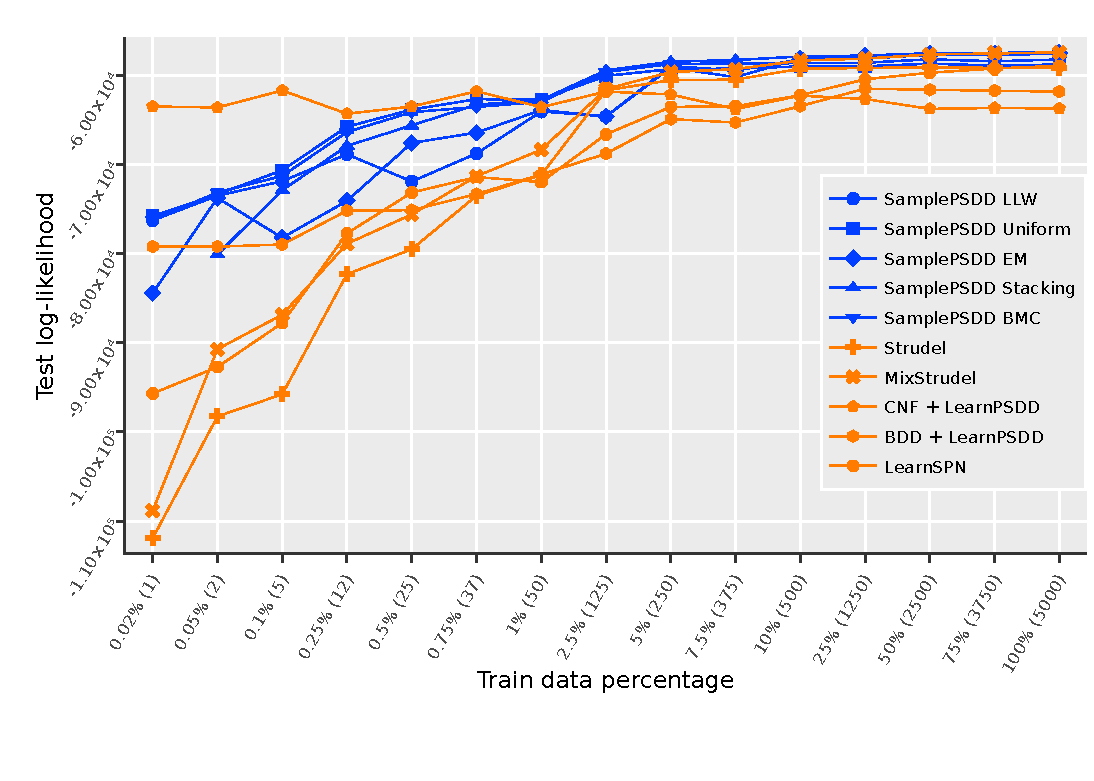
\includegraphics[width=0.765\textwidth]{../plots/bic_ll_led_ensembles.pdf}\\
    \vskip -0.97cm
    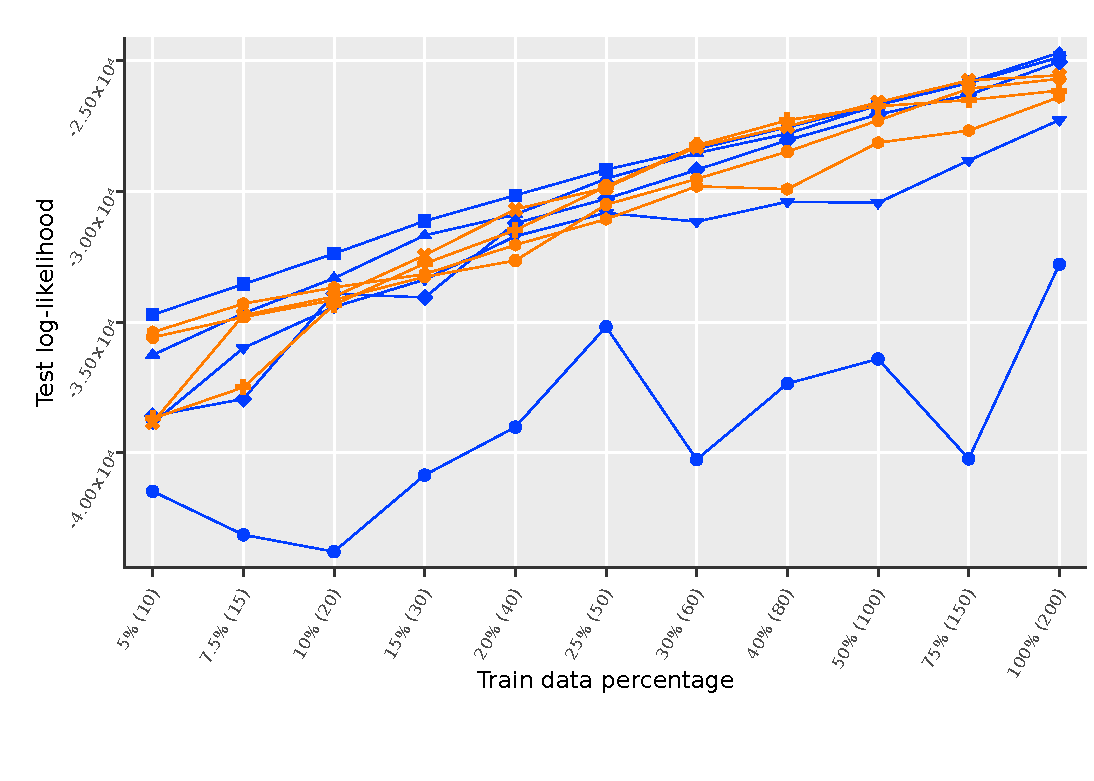
\includegraphics[width=0.765\textwidth]{../plots/bic_ll_led_pixels_ensembles.pdf}
  \end{center}
\end{minipage}}

% Experiments 2
\newpage
\resizebox{0.25\textwidth}{!}{\textcolor{pdblue}{Experiments}}
\vskip 0.25cm
\resizebox{0.495\textwidth}{!}{
\begin{minipage}{0.39\textwidth}
  \noindent
  \colorbox{pyellow}{\textbf{\underline{Evaluation:}}} we sample 30 PSDDs and use 5 ensemble strategies:
  \vskip 0.25cm
  \begin{enumerate}[nosep]
    \item[\llwi]\textcolor{llw}{\textbf{Likelihood weighting (LLW)}},
    \item[\unifi] \textcolor{llw}{\textbf{Uniform weights}},
    \item[\emi] \textcolor{llw}{\textbf{Expectation Maximization (EM)}},
    \item[\stacki] \textcolor{llw}{\textbf{Stacking}},
    \item[\bmci] \textcolor{llw}{\textbf{Bayesian Model Combination (BMC)}};
  \end{enumerate}
  \vskip 0.25cm
  \hskip 0.25cm comparing against \textcolor{unif}{\textbf{\textsc{Strudel}}},
    \textcolor{unif}{\textbf{\textsc{LearnPSDD}}} and \textcolor{unif}{\textbf{\textsc{LearnSPN}}}.
  \vskip 0.25cm
  \colorbox{pyellow}{\textbf{\underline{Datasets:}}} we evaluate with 5 data + knowledge as logic constraints:
  \vskip 0.25cm
  \begin{center}
    \begin{tabular}{cl|rrrr}
      \cline{2-5}
      &\textbf{Dataset} & \textbf{\#vars} & \textbf{\#train} & \textbf{$\phi$'s size}\\
      \cline{2-5}
      &\textsc{LED} & 14 & 5000 & 23 \\
      &\textsc{LED} + \textsc{Images} & 157 & 700 & 39899 \\
      $\Rightarrow$&\textsc{Sushi Ranking} & 100 & 3500 & 17413 \\
      $\Rightarrow$&\textsc{Sushi Top 5} & 10 & 3500 & 37 \\
      &\textsc{Dota 2 Games} & 227 & 92650 & 1308 \\
      \cline{2-5}
    \end{tabular}
  \end{center}
  \begin{align*}
    \text{Our approach }&\text{\colorbox{pblue}{fares \textbf{better} with \textbf{fewer} data}, yet}\\
                        &\text{\colorbox{pgreen}{remains \textbf{competitive} under \textbf{lots of data}}.}
  \end{align*}
  \vskip 0.1cm
  \textcolor{darkgray}{\cite{mattei20,kamishima03,shen17},}

  \textcolor{darkgray}{\cite{choi15,gens13,mei20}}
\end{minipage}}\resizebox{0.495\textwidth}{!}{\begin{minipage}{0.4\textwidth}
  \begin{center}
    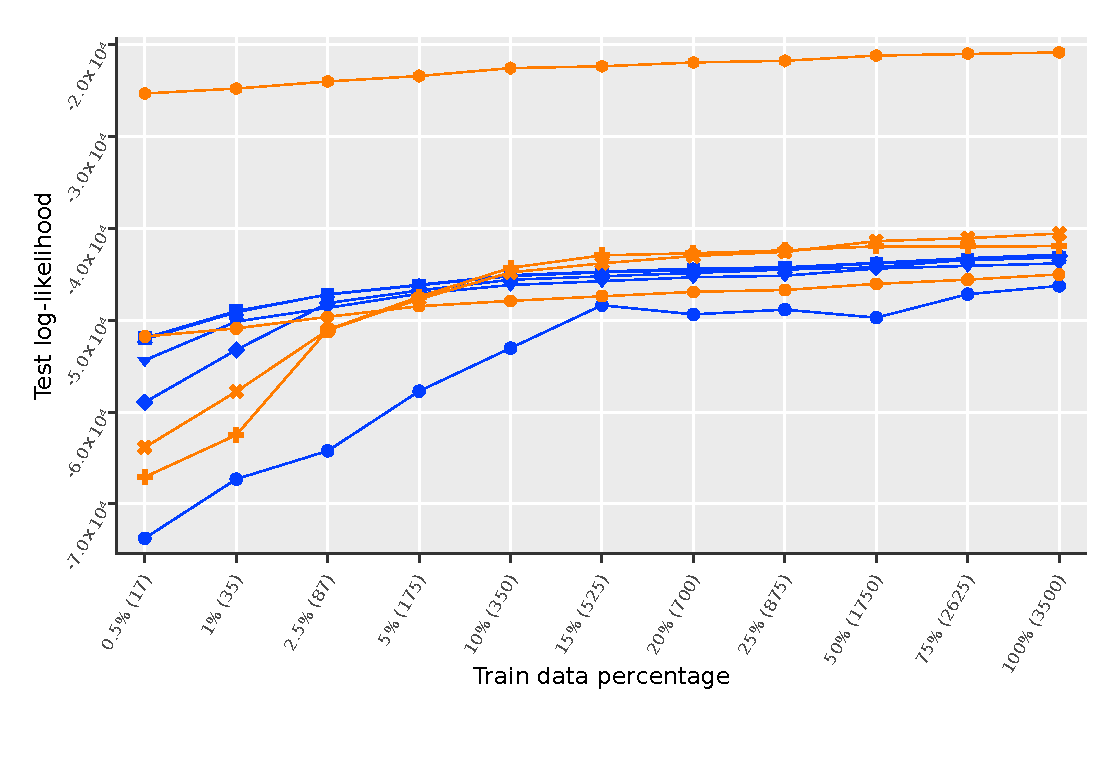
\includegraphics[width=0.765\textwidth]{../plots/bic_ll_sushi_ranking_ensembles.pdf}\\
    \vskip -0.97cm
    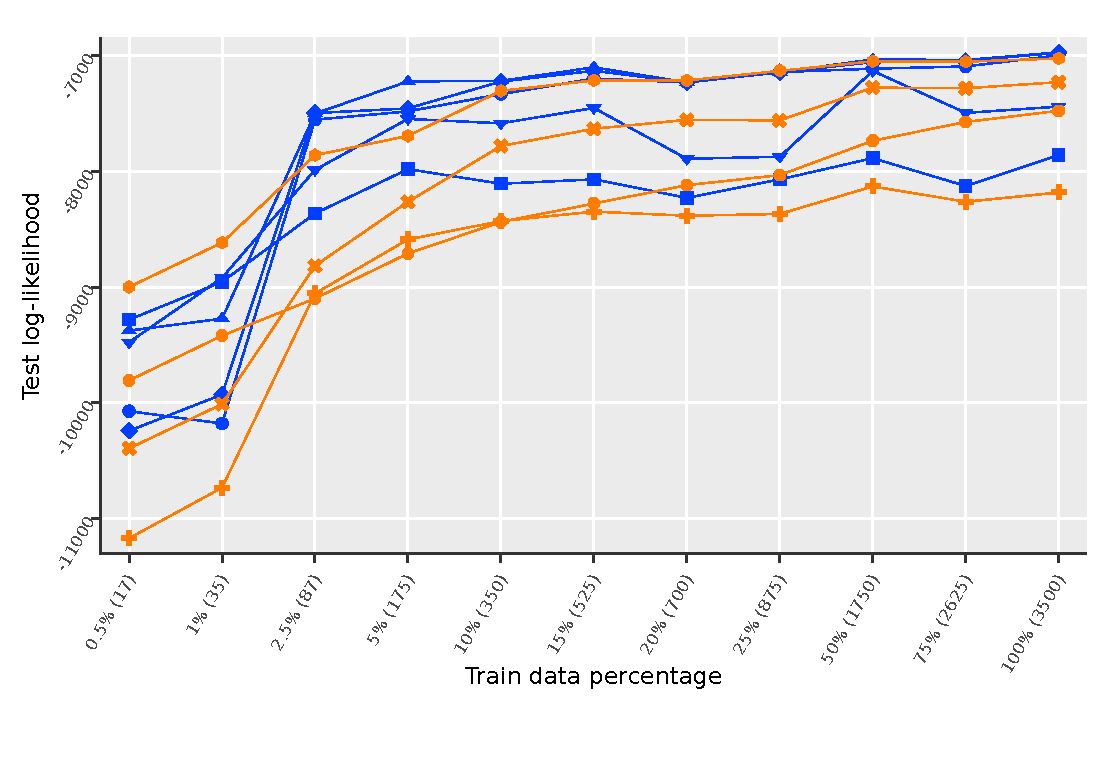
\includegraphics[width=0.765\textwidth]{../plots/bic_ll_sushi_choose_ensembles.pdf}
  \end{center}
\end{minipage}}

% Experiments 3
\newpage
\resizebox{0.25\textwidth}{!}{\textcolor{pdblue}{Experiments}}
\vskip 0.25cm
\resizebox{0.495\textwidth}{!}{
\begin{minipage}{0.39\textwidth}
  \noindent
  \colorbox{pyellow}{\textbf{\underline{Evaluation:}}} we sample 30 PSDDs and use 5 ensemble strategies:
  \vskip 0.25cm
  \begin{enumerate}[nosep]
    \item[\llwi] \textcolor{llw}{\textbf{Likelihood weighting (LLW)}},
    \item[\unifi] \textcolor{llw}{\textbf{Uniform weights}},
    \item[\emi] \textcolor{llw}{\textbf{Expectation Maximization (EM)}},
    \item[\stacki] \textcolor{llw}{\textbf{Stacking}},
    \item[\bmci] \textcolor{llw}{\textbf{Bayesian Model Combination (BMC)}};
  \end{enumerate}
  \vskip 0.25cm
  \hskip 0.25cm comparing against \textcolor{unif}{\textbf{\textsc{Strudel}}},
    \textcolor{unif}{\textbf{\textsc{LearnPSDD}}} and \textcolor{unif}{\textbf{\textsc{LearnSPN}}}.
  \vskip 0.25cm
  \colorbox{pyellow}{\textbf{\underline{Datasets:}}} we evaluate with 5 data + knowledge as logic constraints:
  \vskip 0.25cm
  \begin{center}
    \begin{tabular}{cl|rrrr}
      \cline{2-5}
      &\textbf{Dataset} & \textbf{\#vars} & \textbf{\#train} & \textbf{$\phi$'s size}\\
      \cline{2-5}
      &\textsc{LED} & 14 & 5000 & 23 \\
      &\textsc{LED} + \textsc{Images} & 157 & 700 & 39899 \\
      &\textsc{Sushi Ranking} & 100 & 3500 & 17413 \\
      &\textsc{Sushi Top 5} & 10 & 3500 & 37 \\
      $\Rightarrow$&\textsc{Dota 2 Games} & 227 & 92650 & 1308 \\
      \cline{2-5}
    \end{tabular}
  \end{center}
  \begin{align*}
    \text{Our approach }&\text{\colorbox{pblue}{fares \textbf{better} with \textbf{fewer} data}, yet}\\
                        &\text{\colorbox{pgreen}{remains \textbf{competitive} under \textbf{lots of data}}.}
  \end{align*}
  \vskip 0.1cm
  \textcolor{darkgray}{\cite{mattei20,kamishima03,shen17},}

  \textcolor{darkgray}{\cite{choi15,gens13,mei20}}
\end{minipage}}\resizebox{0.495\textwidth}{!}{\begin{minipage}{0.4\textwidth}
  \begin{center}
    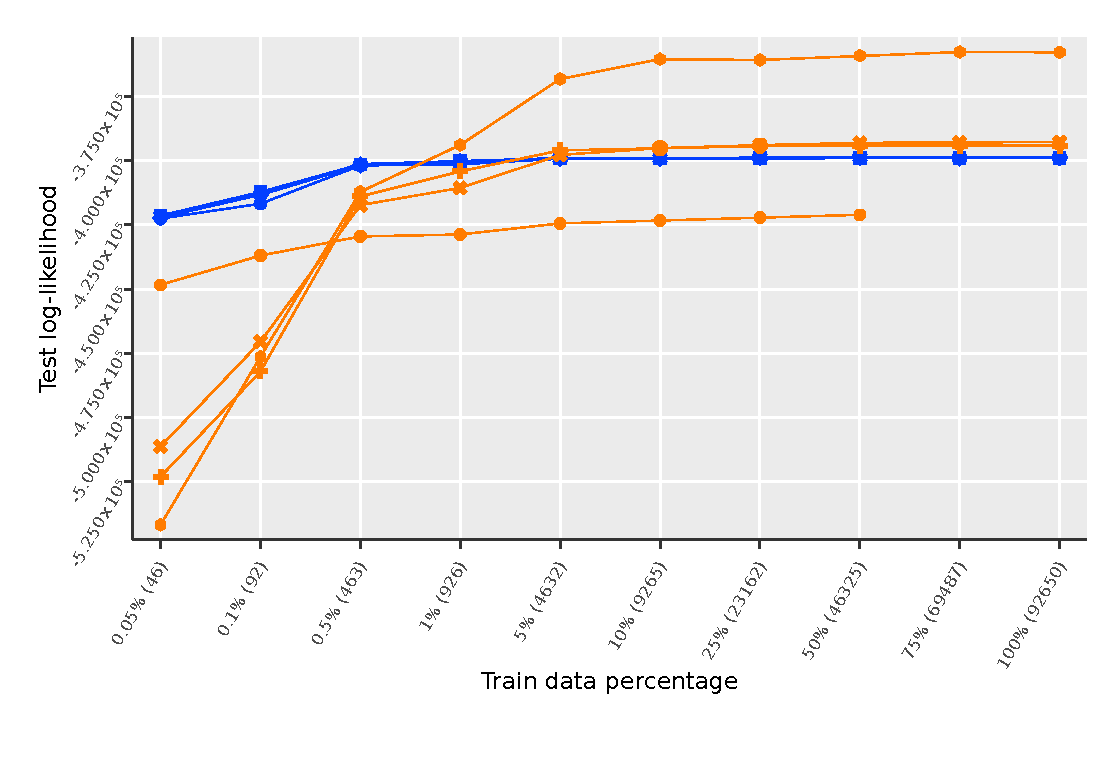
\includegraphics[width=0.765\textwidth]{../plots/bic_ll_dota_ensembles.pdf}\\
    \vskip -0.97cm
    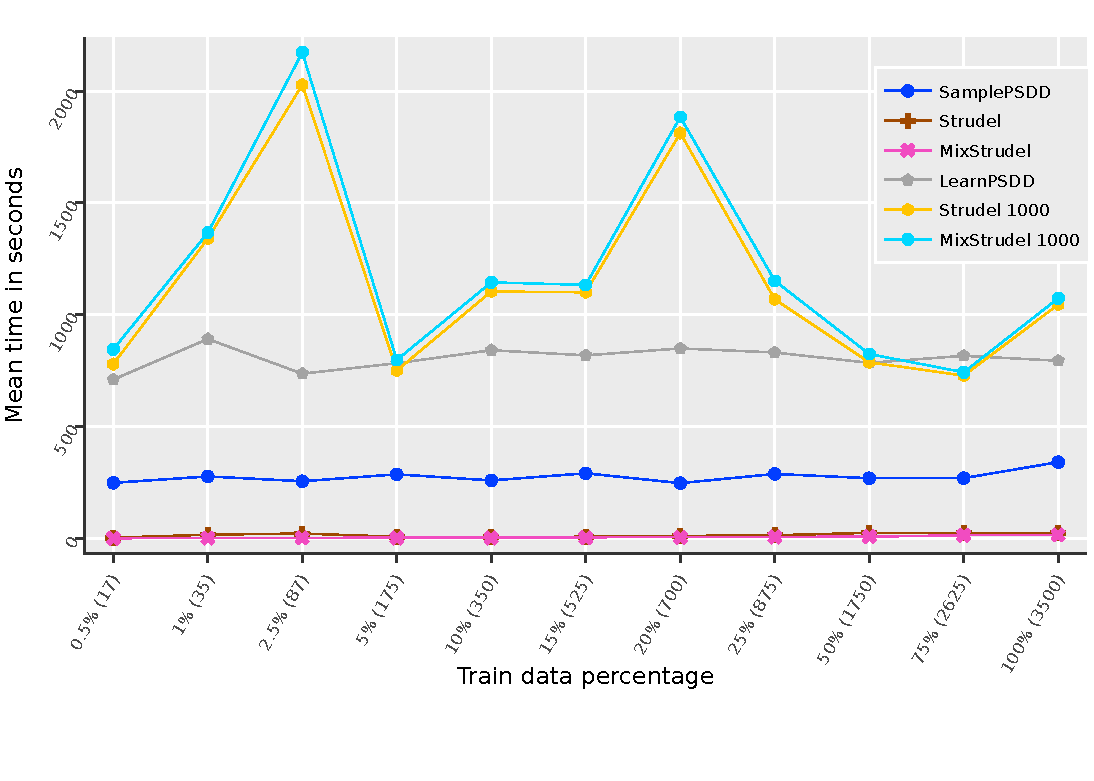
\includegraphics[width=0.765\textwidth]{../plots/all_sushi_time.pdf}
  \end{center}
\end{minipage}}

% Experiments (k, vtree comparison)
\newpage
\resizebox{0.25\textwidth}{!}{\textcolor{pdblue}{Experiments}}
\begin{center}
\vskip -0.7cm
\resizebox{0.4\textwidth}{!}{
  \begin{minipage}{0.35\textwidth}
    \begin{align*}
      \text{What is the impact of }&\text{\colorbox{green}{higher $k$'s} and \colorbox{pyellow}{right-leaning vtrees}}\\
                         \text{in }&\text{\colorbox{pblue}{log-likelihood} and \colorbox{Red}{\color{white}consistency}}?
    \end{align*}
  \end{minipage}
}
\vskip 0.25cm
\begin{center}
  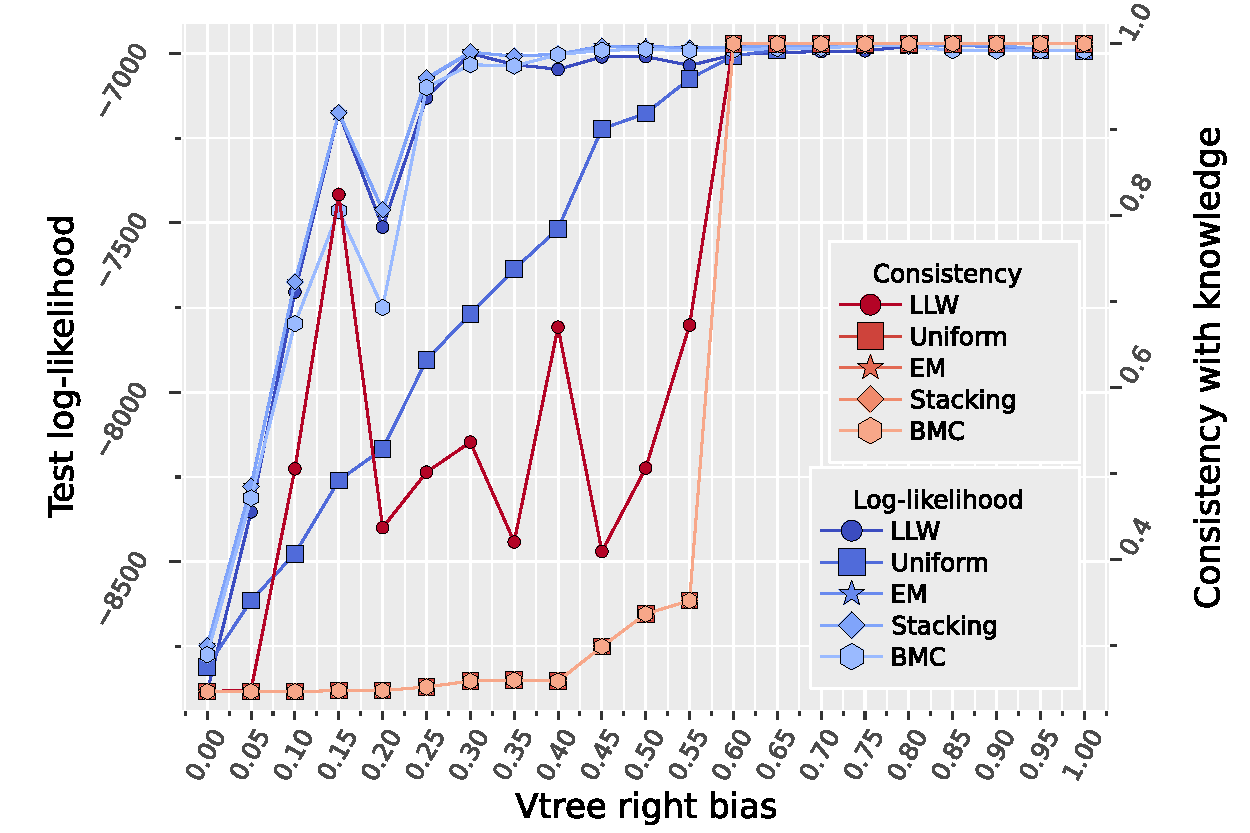
\includegraphics[width=0.3\textwidth]{../plots/vtree_ll_imp_sushi.pdf}
  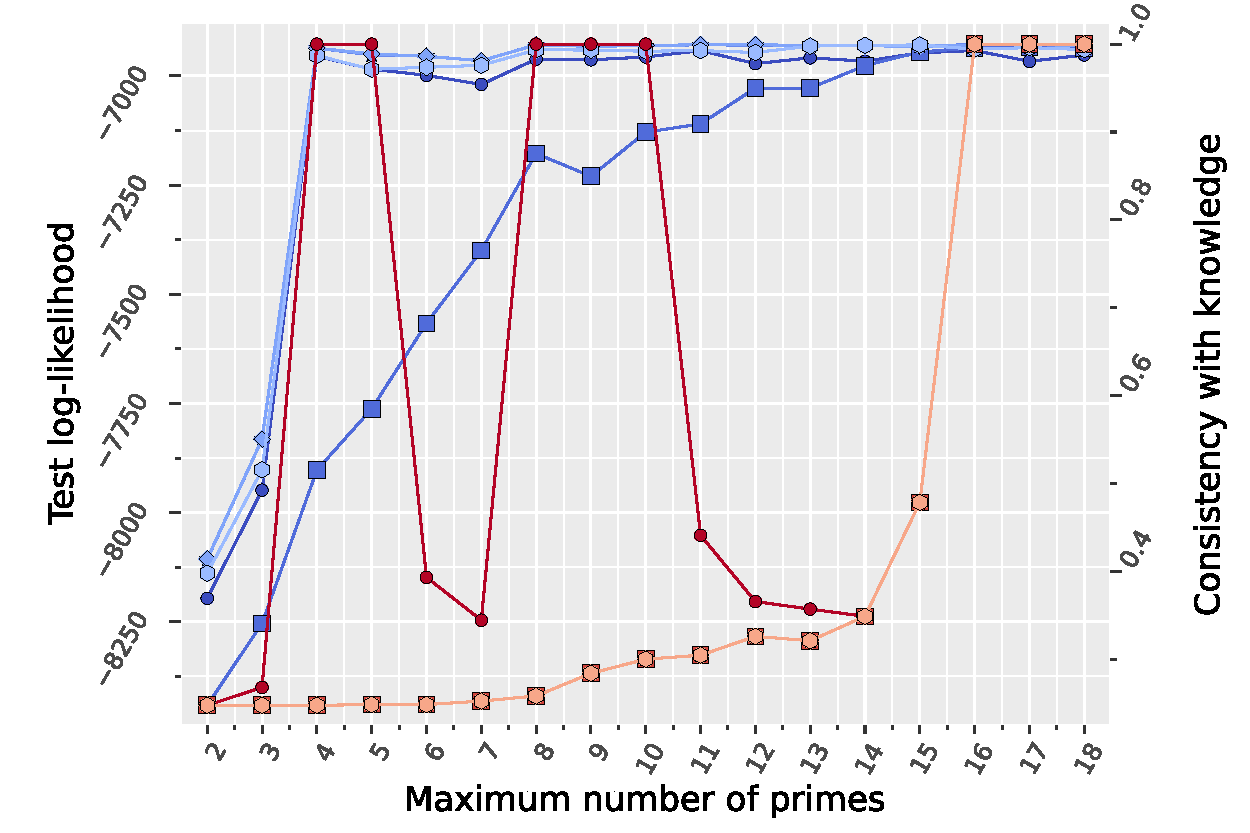
\includegraphics[width=0.3\textwidth]{../plots/k_ll_imp_sushi.pdf}
\end{center}
\vskip -0.5cm
\resizebox{0.4\textwidth}{!}{
  \begin{minipage}{0.4\textwidth}
    \begin{align*}
      \text{Samples perform }&\text{\colorbox{green}{\textbf{better} with higher $k$'s} and \colorbox{pyellow}{right-leaning vtrees}...}\\
                   \text{...}&\text{but at a \colorbox{porange}{\textbf{cost} to complexity}.}
    \end{align*}
  \end{minipage}
}
\begin{center}
  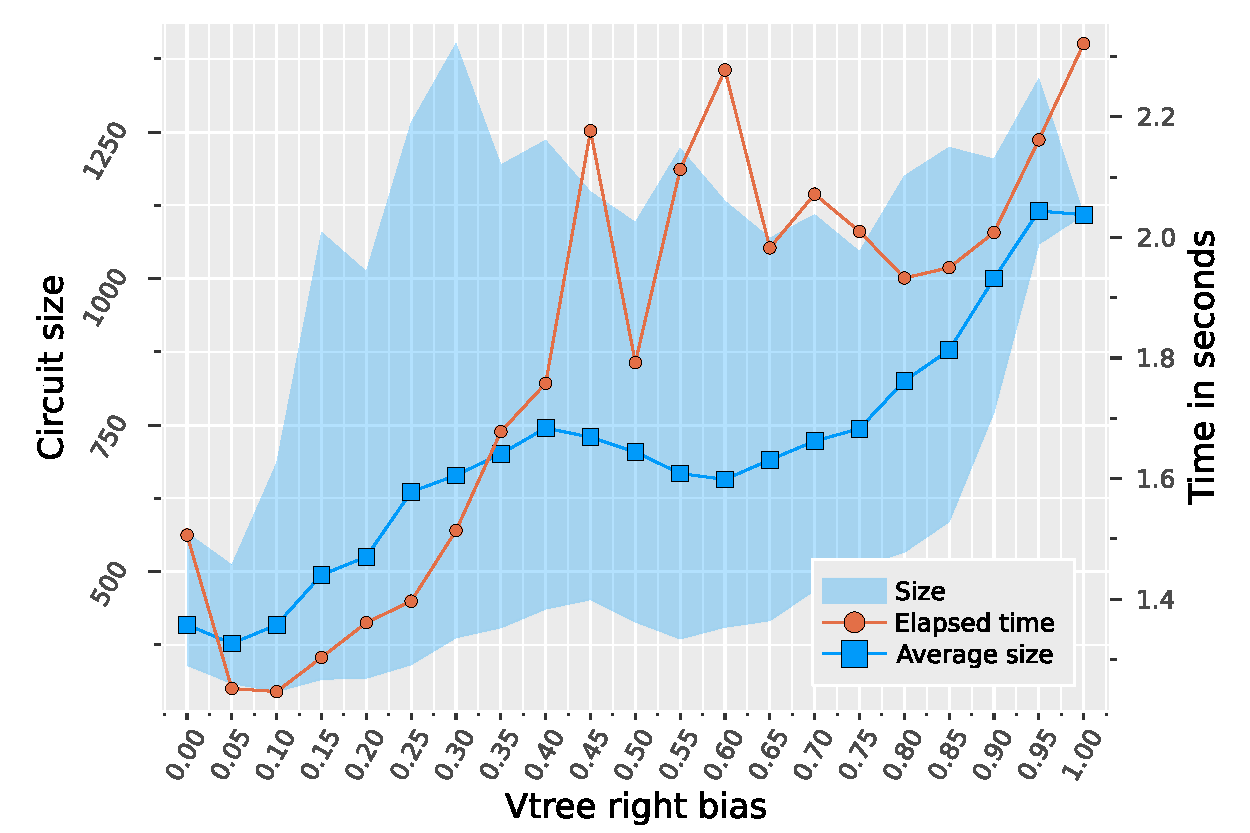
\includegraphics[width=0.3\textwidth]{../plots/vtree_complexity.pdf}
  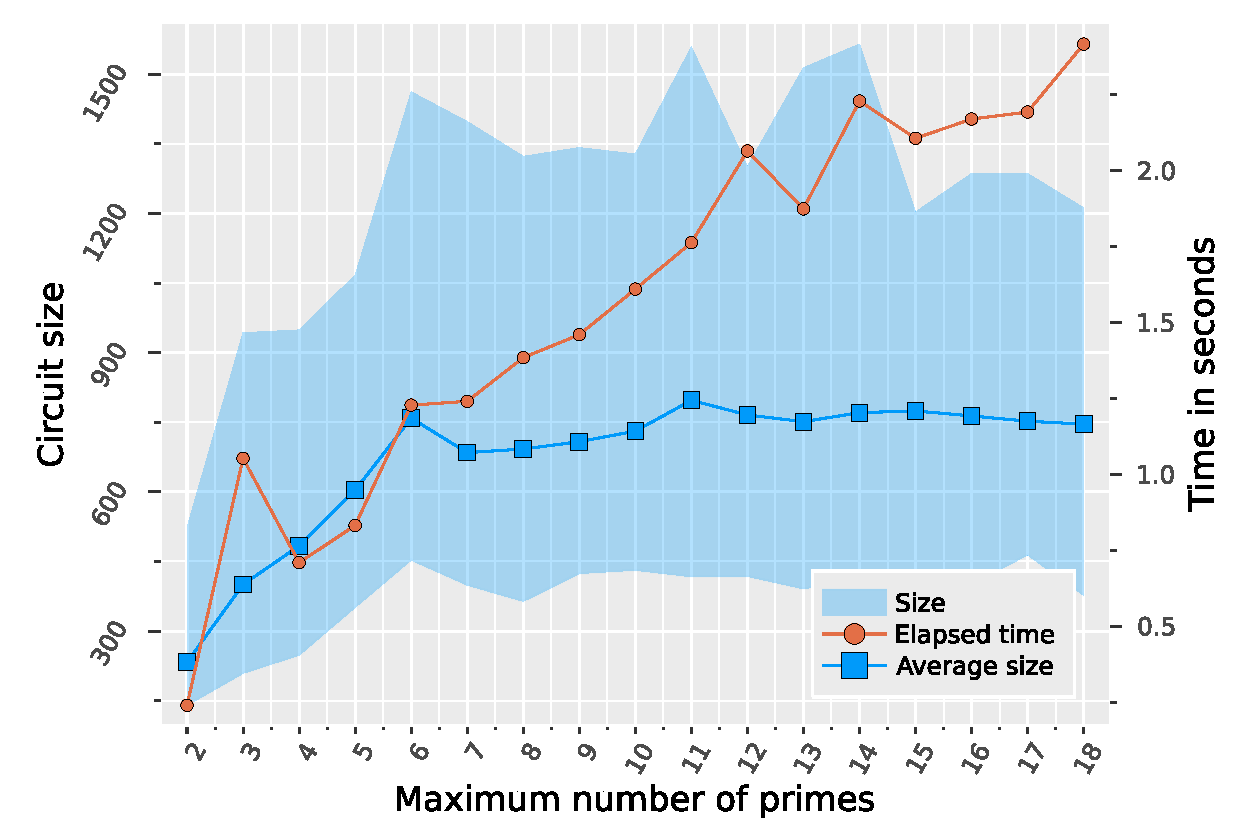
\includegraphics[width=0.3\textwidth]{../plots/k_complexity.pdf}
\end{center}
\end{center}

\nobibliography{../geh_767.bib}

\end{document}
